\chapter{Results and conclusion}
\label{Sect:concl}
\vspace{-0.25em}
As a result of this study, the integral and single-differential cross sections of the reaction $\gamma_{v}p(n) \rightarrow p' (n')\pi^{+}\pi^{-}$ in the kinematic region of invariant mass $W$ from 1.3~GeV to 1.825~GeV and photon virtuality $Q^{2}$ from 0.4~GeV$^2$ to 1~GeV$^2$ were obtained. The cross sections were extracted in the quasi-free regime, which means that FSI-background admixture in the analyzed event sample was decreased as much as was possible and left on a level comparable with that in the free proton cross sections.



%\footnote[1]{Note that in the $\pi^{-}$-missing topology some FSI-background admixture still remains in the quasi-free event sample after the exclusivity cut for $W>1.45$~GeV. This admixture is then corrected as a function of $W$  the following. As the correction due to FSI-background admixture performed for the $\pi^{-}$ topology }.
%Note that FSI-background admixture left after the exclusivity cut in the $\pi^{-}$-missing topology, being corrected only in integral sense, may potentially impact the shape of extracted single-differential distributions (mostly angular). However, since this admixture is present only for events from the $\pi^{-}$-missing topology for $W>$1.45~GeV and stays on the level of 3-7\%, the potential disturbance is anticipated to be less than the total cross section uncertainty.


Figure~\ref{fig:int_w_dep} shows the $W$ dependences of the extracted integral cross sections in various bins in $Q^{2}$, while Figure~\ref{fig:int_q2_dep} shows their $Q^{2}$ dependences in various bins in $W$. The red shadowed area for each point is the total cross section uncertainty, which is the uncertainty $\delta_{\text{stat,mod}}^{\text{tot}}$ (see Sect.~\ref{Sect:mod_dep}) summed up in quadrature with the total systematic uncertainty (see Sect.~\ref{Sect:sys_uncert}). The error bars correspond to the uncertainty $\delta_{\text{stat,mod}}^{\text{tot}}$ only, which for most of the points is smaller than the symbol size.

For each integral ($W$, $Q^{2}$) point nine single-differential cross sections are reported\footnote[1]{Note that FSI-background admixture left after the exclusivity cut in the $\pi^{-}$-missing topology (see Sect.~\ref{Sect:excl_cut_pim_miss}), being corrected only in integral sense, may potentially impact the shape of extracted single-differential distributions (mostly angular). However, since this admixture is present only for events from the $\pi^{-}$-missing topology for $W>$1.4875~GeV and stays on the level of 3-7\%, its impact is not thought to be discernible against the total cross section uncertainty.}. They are presented is App.~\ref{app_cr_sect} with the uncertainty $\delta_{\text{stat,mod}}^{\text{tot}}$ shown by error bars. Once the analysis is approved, the whole set of the extracted cross sections (both integral and single-differential) will be available in the CLAS physics database~\cite{CLAS_DB}.


%\afterpage{\clearpage}

\begin{figure}[htp]
\begin{center}
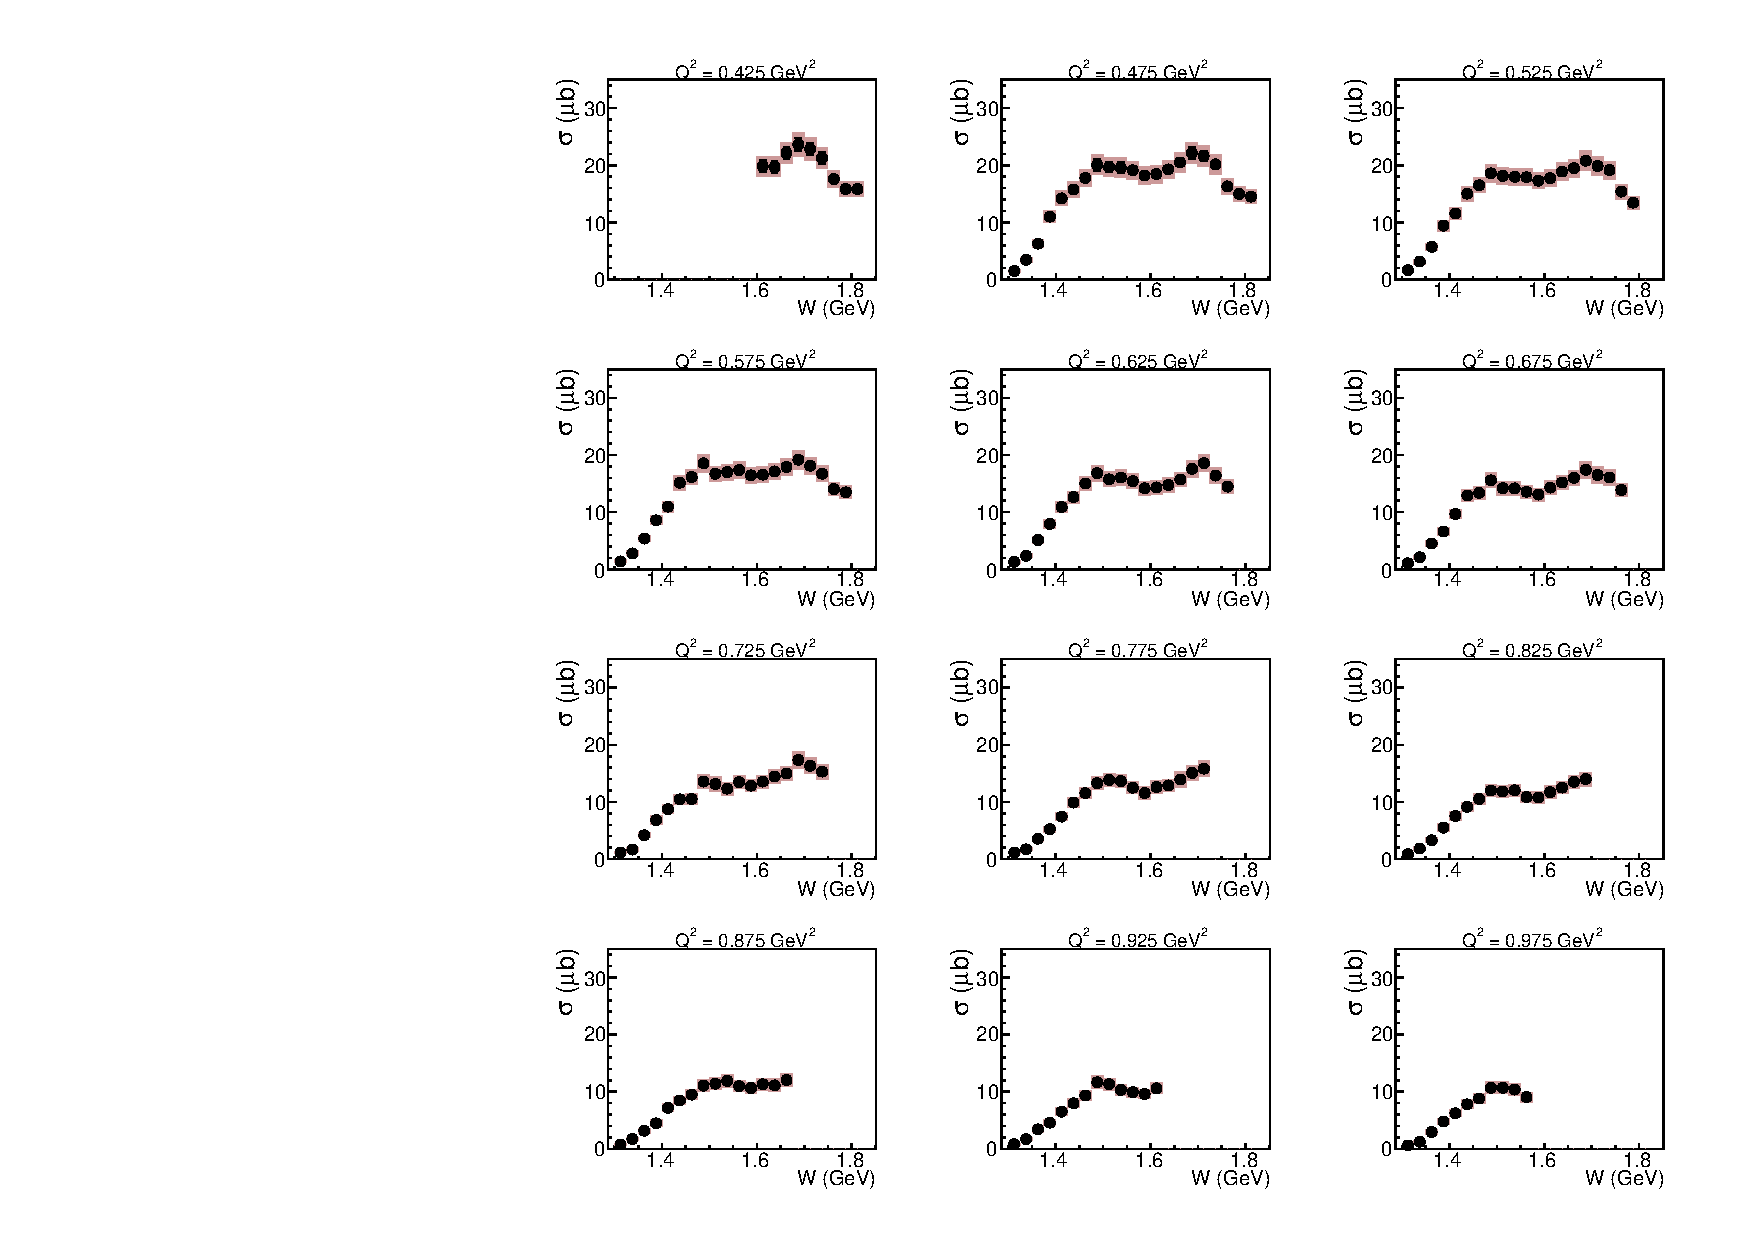
\includegraphics[width=\textwidth]{pictures/conclusion/w_dep_new.pdf}
\caption{\small $W$ dependences of the extracted integral cross sections in various bins in $Q^{2}$. The pink shadowed area for each point is the total cross section uncertainty, which is the uncertainty $\delta_{\text{stat,mod}}^{\text{tot}}$ (see Sect.~\ref{Sect:mod_dep}) summed up in quadrature with the total systematic uncertainty (see Sect.~\ref{Sect:sys_uncert}). The error bars that correspond to the uncertainty $\delta_{\text{stat,mod}}^{\text{tot}}$ only, are smaller than the symbol size.   } \label{fig:int_w_dep}
\end{center}
\end{figure}


\begin{figure}[htp]
\begin{center}
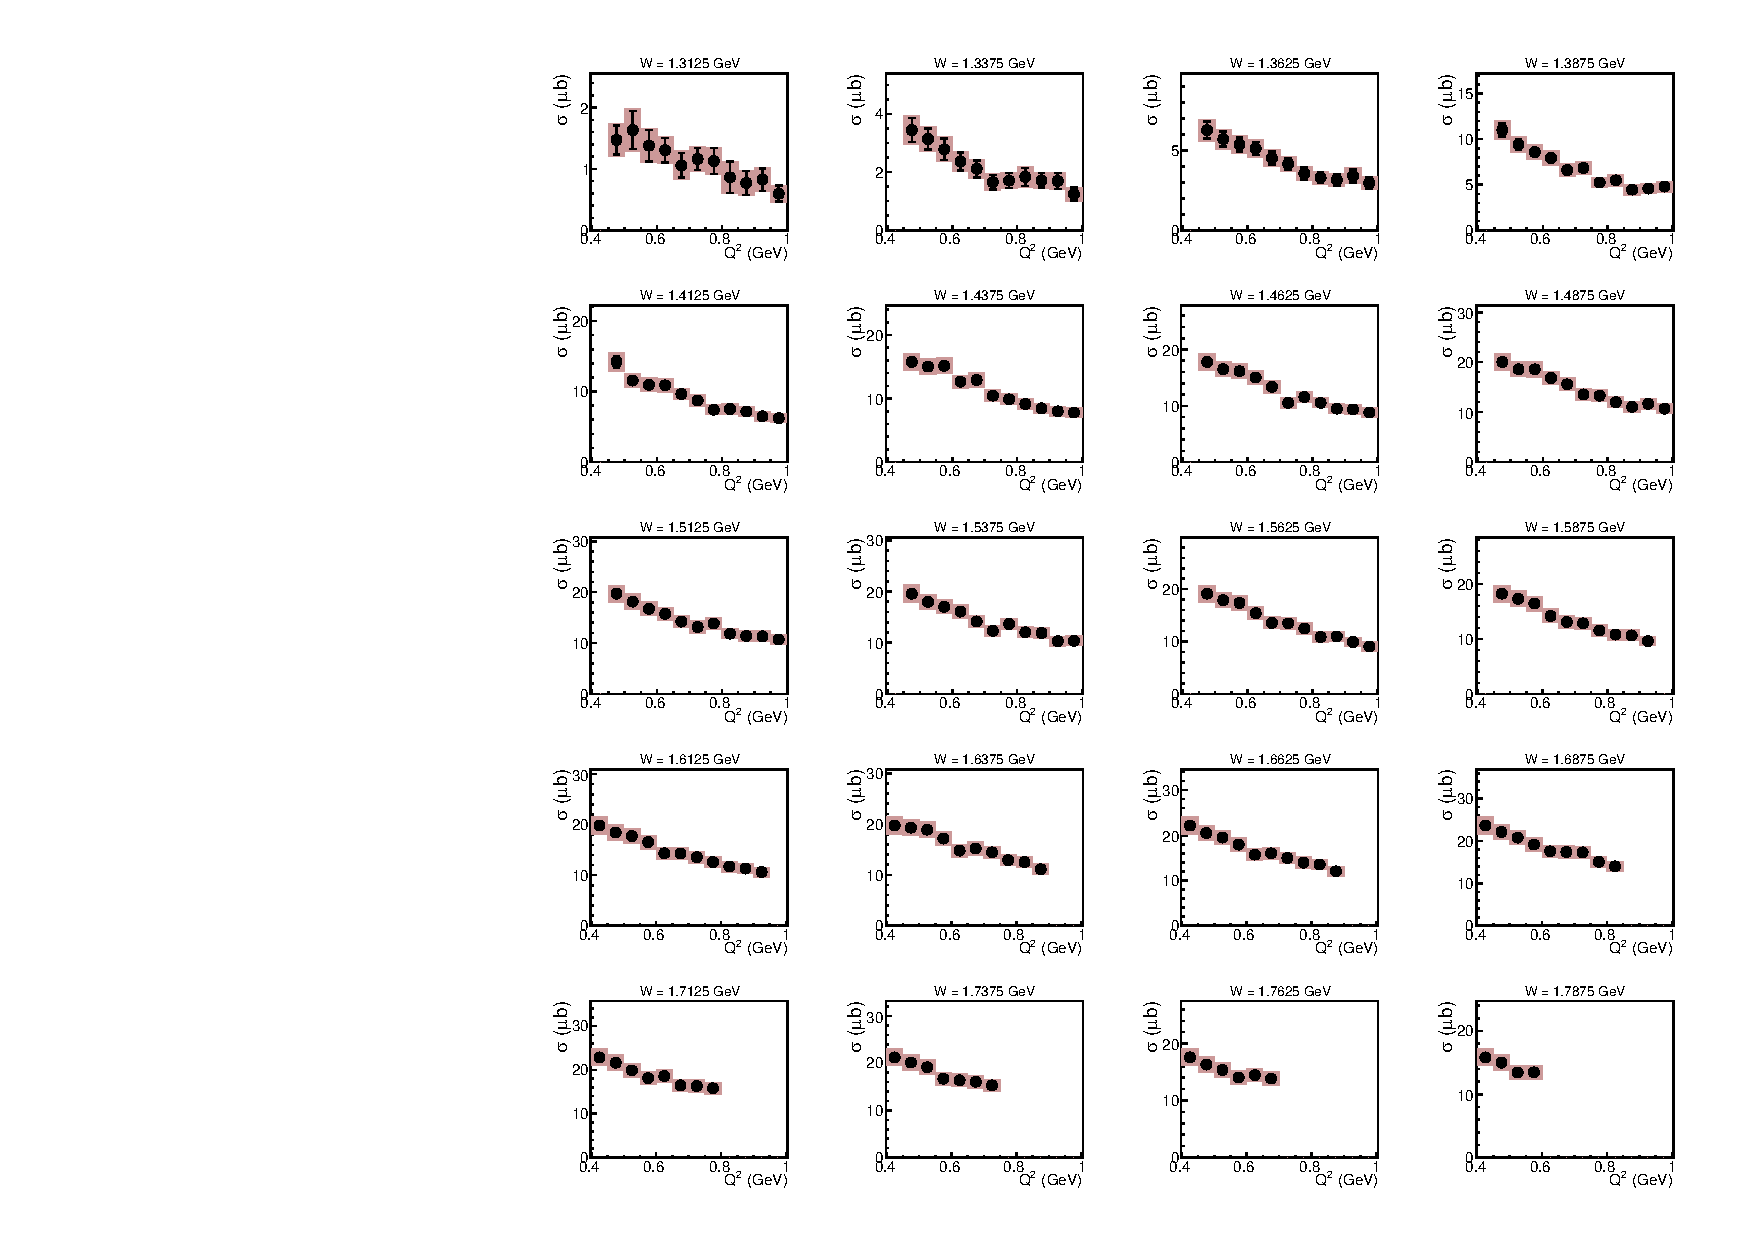
\includegraphics[width=\textwidth]{pictures/conclusion/q2_dep_new.pdf}
\caption{\small $Q^{2}$ dependences of the extracted integral cross sections in various bins in $W$. The pink shadowed area for each point is the total cross section uncertainty, which is the uncertainty $\delta_{\text{stat,mod}}^{\text{tot}}$ (see Sect.~\ref{Sect:mod_dep}) summed up in quadrature with the total systematic uncertainty (see Sect.~\ref{Sect:sys_uncert}). The error bars that correspond to the uncertainty $\delta_{\text{stat,mod}}^{\text{tot}}$ only, are smaller than the symbol size.  } \label{fig:int_q2_dep}
\end{center}
\end{figure}


After approval the cross sections will be subject to further physical interpretation, which includes as an important step the comparison with the double-pion cross sections off the free proton recently extracted from CLAS data~\cite{Fed_an_note:2017,Fed_paper_2018}. These cross sections were obtained in the same experimental configuration (including beam energy and target setup) as the cross sections of this study. Both measurements have, therefore, similar inherent systematic inaccuracies. Moreover, the cross sections of both sets, being obtained in the same kinematic region, have identical binning in the kinematic variables that advantages their direct comparison. This comparison hence provides the experimentally best possible opportunity to investigate the differences and alterations (including possible in-medium modifications) that occur in the exclusive reaction off the bound proton in comparison with that off the free proton.

\begin{figure}[htp]
\begin{center}
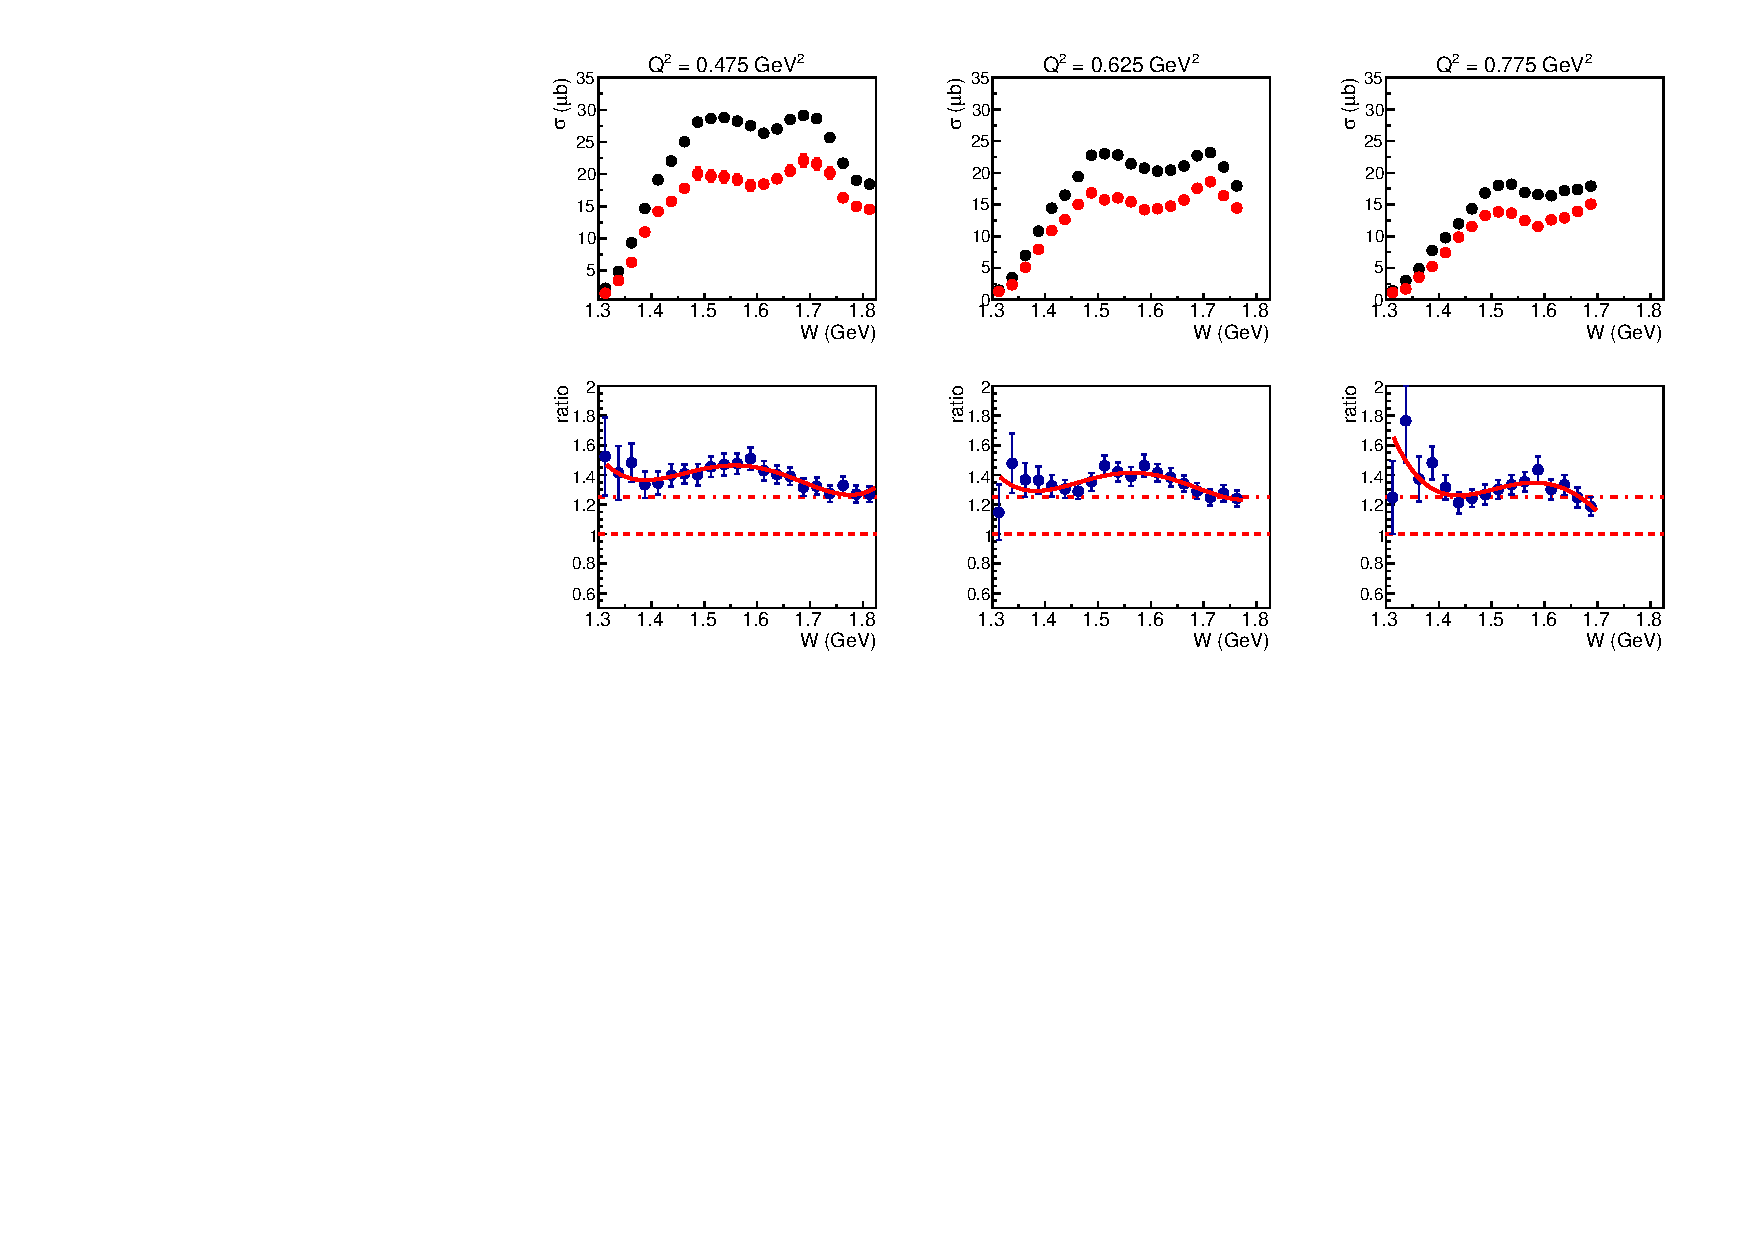
\includegraphics[width=\textwidth]{pictures/conclusion/with_fed_comp.pdf}
\caption{\small Comparison between integral cross sections obtained in this analysis (red symbols) and those obtained off the free proton~\cite{Fed_an_note:2017,Fed_paper_2018} (black symbols) shown for three typical equidistant $Q^{2}$ bins specified in the plots. The cross sections from both studies are given with the uncertainties $\delta_{\text{stat,mod}}^{\text{tot}}$ only (shown by error bars), while systematic effects are assumed to be identical and are hence ignored. The bottom row of Fig.~\ref{fig:int_q2_dep} shows the ratio of the corresponding distributions from the top row together with its preliminary fit by the fifth order polynomial. The dashed line marks the position of unity, while the dash-dotted line shows the value of 1.25. } \label{fig:int_q2_dep}
\end{center}
\end{figure}

The top row of Fig.~\ref{fig:int_q2_dep} shows some example plots, which demonstrate the difference between integral cross sections obtained in this analysis (red symbols) and their free proton analogue from Ref.~\cite{Fed_an_note:2017,Fed_paper_2018} (black symbols). The comparison shown here is given for three typical equidistant $Q^{2}$ bins specified in the plots. The cross sections from both studies are given with the uncertainties $\delta_{\text{stat,mod}}^{\text{tot}}$ only (shown by error bars), while systematic effects are assumed to be identical and are hence ignored. The bottom row of Fig.~\ref{fig:int_q2_dep} shows the ratio of the corresponding distributions from the top row together with its preliminary fit by the fifth order polynomial.

%The top row of Fig.~\ref{fig:int_q2_dep} shows a preliminary comparison between integral cross sections of this analysis (red symbols) and those obtained off the free proton~\cite{Fed_an_note:2017,Fed_paper_2018} (black symbols).


The examples shown in Fig.~\ref{fig:int_q2_dep} indicate a pronounced difference between the free proton cross section and its quasi-free analogue measured off the proton bound in deuterium. This difference, which is thought to be attributed mainly to the FSI effects, is seeking a detailed investigation and physical interpretation including the study of its dependence on various kinematic variables. This activity will eventually shed light on the processes that occur in the deuteron, such as FSI and in-medium effects.

Further physical discussions and interpretations of the obtained results are left for the PhD thesis (which is in preparation) and a future publication on the subject.


It is also noteworthy that during this study a sophisticated analysis framework was elaborated that includes the tools for data processing and cross section calculation. This framework, which is partially based on the achievements of the study~\cite{Fed_an_note:2017,Fed_paper_2018}, might be of use for future studies including the upcoming analysis of new CLAS12 data. Therefore, the data analysis procedure and the links to the codes of programs and scripts are given in App.~\ref{app_code}.



